% concatenated from main.tex
% Default LaTeX template.
\documentclass{article}

\newcommand{\prox}{\operatorname{prox}}

\usepackage[T1]{fontenc}
\usepackage[utf8]{inputenc}
\usepackage{amsmath,amssymb,mathtools,amsthm}
% \usepackage[expansion=false]{microtype}
% \usepackage[margin=1.15in]{geometry}
\usepackage[hidelinks]{hyperref}
\usepackage{tikz}
\newtheorem{theorem}{Theorem}[section]
\newtheorem{proposition}[theorem]{Proposition}
\newtheorem{lemma}[theorem]{Lemma}
\newtheorem{corollary}[theorem]{Corollary}
\theoremstyle{remark}
\newtheorem{remark}[theorem]{Remark}
\usepackage{pgfplots}
\pgfplotsset{compat=1.18}


\DeclareMathOperator*{\argmin}{argmin}
\newcommand{\Lip}{\operatorname{Lip}}
\newcommand{\R}{\mathbb{R}}
\newcommand{\C}{\mathbb{C}}

\newcommand{\norm}[1]{\| #1\|}
\newcommand{\ip}[2]{\langle #1,#2\rangle}
\newcommand{\dd}{\,\mathrm{d}}
\raggedbottom
\emergencystretch=2em

\title{
Nesterov Flow May Travel Infinitely Long to Converge to a Minimizer
}
\author{Ernest K. Ryu}
\date{}

\begin{document}

\maketitle

\begin{abstract}
Recent work has established that the trajectory of the Nesterov ODE, a the continuous-time model of Nesterov's accelerated gradient method, exhibits point convergence towards a minimizer of a convex potential. A natural next question is whether this point convergence can be upgraded to rectifiability, namely whether the convergent orbit has finite path length. This work provides the answer in the negative by constructing a differentiable convex potential in $\mathbb{R}^2$ for which the flow converges to its minimizer but still accumulates infinite path length. All proofs of this work are due entirely to an internal model at OpenAI.
\end{abstract}


\section{Introduction}

The critical Nesterov flow
\[
  \ddot X(t)+\frac{3}{t}\dot x(t)+\nabla f(x(t))=0
  \qquad t>0
\]
with initial condition $X(0)=X_0$ and $\dot{X}(0)=0$ and differentiable convex function $f\colon\mathbb{R}^d\rightarrow\mathbb{R}$ was introduced by Su, Boyd, and Cand\`es \cite{SuBoydCandes2014,SuBoydCandes2016} as the continuous-time model of Nesterov's accelerated gradient method \cite{Nesterov1983}. 
A Lyapunov analysis yields the function-value rate
\[
  f(X(t)) - \min f = \mathcal{O}(1/t^2),
\]
and a large body of literature has studied finer asymptotic properties of the Nesterov flow \cite{attouch2000heavy,chambolle2015convergence,attouch2015fast,attouch2016fast,may2017asymptotic,AttouchChbaniPeypouquetRedont2018,attouch2019rate,attouch2025recovering}. Most recently, Jang, Ryu, Bo{\c t}, Fadili, and Nguyen 
 proved that the trajectory itself converges to a minimizer if a minimizer exists \cite{JangRyu2025,BotFadiliNguyen2025}.



There is also an active body of work bounding the path length for gradient flow $\dot{X}=-\nabla f(X)$ based on the Kurdyka--{\L}ojasiewicz (KL) inequality \cite{Lojasiewicz1963,Kurdyka1998,BolteDaniilidisLeyMazet2010,AbsilMahonyAndrews2005,AttouchBolteRedontSoubeyran2010,AttouchBolteSvaiter2013,AttouchChbaniPeypouquetRedont2018,AttouchChbaniRiahi2019,DAcuntoKurdyka2021}
and the notion of self-contracting curves 
\cite{ManselliPucci1991,DaniilidisLeySabourau2010,DaniilidisDavidDurandCartagenaLemenant2015,StepanovTeplitskaya2017,GuptaBalakrishnanRamdas2021}.


% Path-length estimates for first-order gradient dynamics are often obtained through the Kurdyka--{\L}ojasiewicz (KL) framework. The foundational gradient inequality goes back to {\L}ojasiewicz's real-analytic setting \cite{Lojasiewicz1963}, was extended by Kurdyka to definable functions \cite{Kurdyka1998}, and was further characterized for subgradient flows in tame nonsmooth settings \cite{BolteDaniilidisLeyMazet2010}. In optimization, this line yields finite-length convergence for broad descent/proximal schemes \cite{AbsilMahonyAndrews2005,AttouchBolteRedontSoubeyran2010,AttouchBolteSvaiter2013}, and for related inertial systems \cite{AttouchChbaniPeypouquetRedont2018,AttouchChbaniRiahi2019}. Quantitative variants also provide explicit length bounds in structured classes such as polynomials and definable families \cite{DAcuntoKurdyka2021}.

% A complementary geometric line exploits self-contractedness of convex-gradient trajectories. In the plane, rectifiability of steepest-descent curves was proved by Manselli and Pucci \cite{ManselliPucci1991}; this was extended to higher-dimensional Euclidean spaces \cite{DaniilidisLeySabourau2010,DaniilidisDavidDurandCartagenaLemenant2015} and then to arbitrary finite-dimensional normed spaces \cite{StepanovTeplitskaya2017}. Recent optimization-focused work also establishes upper and lower path-length bounds for gradient flow and gradient descent under broad assumptions \cite{GuptaBalakrishnanRamdas2021}.



For the critical Nesterov flow, a natural next question is whether this point convergence can be upgraded to \emph{rectifiability}, namely whether the convergent orbit has finite path length. This paper presents the answer in the negative. We construct a convex $C^1$ potential $f\colon \mathbb{R}^2\rightarrow\mathbb{R}$ for which the flow converges to its minimizer but still accumulates infinite path length.



The construction is based on two key insights. First, for radial potentials, the associated flow satisfies a conservation-of-angular-momentum-like identity:
\[
  t^3
  \!\!\!
\underbrace{
  \det\big(x(t),\dot x(t)\big)}_{=\text{angular momentum}}\!\!\equiv \kappa,.
\]
Second, the pathology arises when the potential behaves like $\|x\|$ near the origin. But, to ensure differentiability at the origin, we have the gradient vanish slowly (logarithmically) as $x\rightarrow 0$.

\paragraph{Comment on the use of AI.} The mathematical proofs in this paper are due entirely to an internal model at OpenAI. The role of the human author was simply to digest the proofs and modify the write-ups for clarity.



% We then add a localized convex anisotropic perturbation near the initial point. This perturbation acts only for a finite time, but it creates nonzero angular momentum. Once the trajectory has entered a sufficiently small neighborhood of the minimizer, the perturbation vanishes identically and the motion is governed again by the radial potential alone. The resulting tail has conserved angular momentum, and the combination of
% \[
%   \| x(t)\|\lesssim \frac{\log t}{t^2}
%   \qquad\text{and}\qquad
%   t^3\det\bigl(x(t),\dot x(t)\bigr)\equiv \kappa\neq0
% \]
% forces the tangential velocity to behave like $1/(t\log t)$, which is not integrable.
% XXXX
% The same analysis also yields two comparison results that clarify the mechanism. First, if $f$ is quadratic and the trajectory is started from regular data $x(0)=x_0$, $\dot x(0)=0$, then each spectral mode solves a Bessel equation, every orbit is rectifiable, and the objective values decay like $O(t^{-3})$. Thus the nonrectifiable phenomenon is not already present in the linearized regime. Second, for the first-order gradient flow $\dot y=-\nabla f(y)$ associated with the radial core potential, every trajectory is radial and has total length exactly $\| y(0)\|$; in fact the minimizer is reached in finite time. Hence the infinite-length behavior is genuinely tied to the second-order inertial dynamics.



\section{Construction with infinite path length}

In this section, we prove the following principal claim.

\begin{theorem}\label{thm:main}
There exist a convex $C^1$ function $f\colon\R^2\to\R$ with unique minimizer at the origin and a global solution $X\colon[0,\infty)\to\R^2$ of
\[
   \ddot X(t)+\frac{3}{t}\dot X(t)+\nabla f(X(t))=0,
  \qquad t>0,
  \qquad X(0)=X_0,
  \qquad \dot X(0)=0,
\]
some $X_0\neq0$, 
such that
% \[
%   X(t)\to0
%   \qquad\text{as }t\to\infty,
% \]
% but
\[
  \int_0^\infty \| \dot X(t)\|\,\dd t=\infty.
\]
\end{theorem}


\subsection{Almost radial construction}

\begin{figure}[t]
\centering
\hspace{-0.3in}
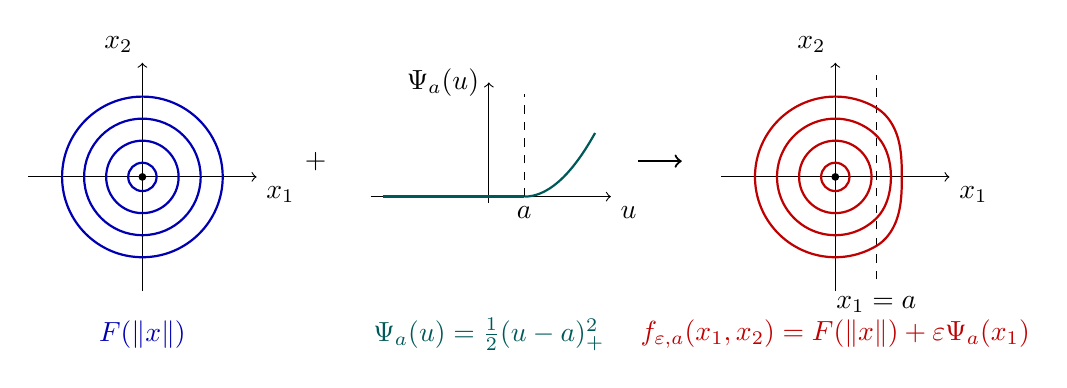
\begin{tikzpicture}[scale=1]
  % Left panel: radial core F(|x|)
  \begin{scope}[shift={(-4.4,0)}]
    \draw[->] (-1.45,0) -- (1.45,0) node[below right] {$x_1$};
    \draw[->] (0,-1.45) -- (0,1.45) node[above left] {$x_2$};
    \foreach \r in {0.18,0.46,0.74,1.02} {
      \draw[blue!70!black,thick] (0,0) circle (\r);
    }
    \fill (0,0) circle (1.4pt);
    \node[blue!70!black] at (0,-2.0) {$F(\|x\|)$};
  \end{scope}

  % Middle panel: one-sided perturbation Psi(x_1)
  \begin{scope}[shift={(0,-0.25)}]
    \draw[->] (-1.5,0) -- (1.55,0) node[below right] {$u$};
    \draw[->] (0,-0.08) -- (0,1.45) node[left] {$\Psi_a(u)$};
    \draw[dashed] (0.45,0) -- (0.45,1.3);
    \node[below] at (0.45,0) {$a$};
    \draw[teal!70!black,thick] (-1.35,0) -- (0.45,0);
    \draw[teal!70!black,thick,samples=120,domain=0.45:1.35,smooth]
      plot (\x,{1.0*(\x-0.45)^2});
    \node[teal!70!black] at (0,-1.75) {$\Psi_a(u)=\frac12(u-a)_+^2$};
  \end{scope}

  % Right panel: combined level sets of f_eps
  \begin{scope}[shift={(4.4,0)}]
  \def\a{0.52}
  \draw[->] (-1.45,0) -- (1.45,0) node[below right] {$x_1$};
  \draw[->] (0,-1.45) -- (0,1.45) node[above left] {$x_2$};
  \draw[dashed] (\a,-1.3) -- (\a,1.3);
  \node[below] at (\a,-1.4) {$x_1=a$};

  % Concentric rings near the origin (radial region)
  \foreach \rr in {0.18,0.46} {
    \draw[red!75!black,thick] (0,0) circle (\rr);
  }

  % Outer level sets deformed only after crossing x_1=a
  \foreach \rr in {0.74,1.02} {
    \draw[red!75!black,thick,samples=200,smooth,domain=0:360,variable=\t]
      plot ({(\rr - 0.7*(max(\rr*cos(\t)-\a,0))^2)*cos(\t)},
            {(\rr - 0.7*(max(\rr*cos(\t)-\a,0))^2)*sin(\t)});
  }

  \fill (0,0) circle (1.4pt);
  \node[red!75!black] at (0,-2.0)
    {$f_{\varepsilon,a}(x_1,x_2)=F(\|x\|)+\varepsilon\Psi_a(x_1)$};
\end{scope}

  % Plus and arrow annotations
  \node at (-2.2,0.2) {$+$};
  \draw[->,thick] (1.9,0.2) -- (2.45,0.2);
\end{tikzpicture}
\caption{Illustration of the potential $f_{\varepsilon,a}$. The function is radial near the origin, while the one-sided quadratic perturbation $\varepsilon\Psi_a(x_1)$, whose purpose is to generate positive angular momentum, becomes inactive once the trajectory is sufficiently close to the origin.
}
\label{fig:feps-schematic}
\end{figure}



Define $F\colon[0,\infty)\to\R$ by
\[
  F(0)=0,
  \qquad
  F(r)=
  \begin{cases}
    \displaystyle \int_0^r \frac{\dd u}{-\log u}, & 0<r\le e^{-2},\\[6pt]
    F(e^{-2})+\tfrac12\bigl(r-e^{-2}\bigr), & r\ge e^{-2}.
  \end{cases}
\]
Let $a>0$ and $\varepsilon>0$. Define
\[
  \Psi_a(u)=\frac12 (u-a)^2_+,
  \qquad
  (u-a)_+=\max\{u-a,0\}
  \]
and
\[
   f_{\varepsilon,a}(x_1,x_2)
  =
  F\Big(\sqrt{x_1^2+x_2^2}\Big)+\varepsilon \Psi_a(x_1).
\]
See Figure~\ref{fig:feps-schematic} for an illustration of $f_{\varepsilon,a}$.
From direct calculations, it can be checked that $f_{\varepsilon,a}\colon\mathbb{R}^2\rightarrow\mathbb{R}$ is convex and continuously differentiable, and $0$ is its unique minimizer of $f_{\varepsilon,a}$.

Let $\{X(t)\}_{t\ge 0}$ be the solution to
\[
   \ddot X(t)+\frac{3}{t}\dot X(t)+\nabla f_{\varepsilon,a}(X(t))=0,
  \qquad t>0,
  \qquad X(0)=(2a,a),
  \qquad \dot X(0)=0.
\]
Since the minimizer is unique, the convergence results of prior work imply $X(t)\rightarrow 0$. 
We refer to 
\[
\{x\in \mathbb{R}^2:\|x\|\le a\}
\]
as the \emph{radial region} since $f_{\varepsilon,a}(x)=F(\|x\|)$ is radial in this region. 
Note that the initial point $X(0)=(2a,a)$ is outside of the radial region.
Let
\begin{equation*}
T_\mathrm{rad}=\sup\{t: \|X(t)\|> a\}
% \label{eq:enter-time}  
\end{equation*}
be the time at which the dynamics $\{X(t)\}_{t\ge 0}$ permanently enters the radial region. Since $X(t)\rightarrow 0$, we have $T_\mathrm{rad}<\infty$.




% \begin{lemma}\label{prop:potential}
% The function $f_{\varepsilon,a}\colon\mathbb{R}^2\rightarrow\mathbb{R}$ is convex and continuously differentiable. Moreover, $0$ is its unique minimizer.
% \end{lemma}
% \begin{proof}
% Follows from straightforward calculations.
% \end{proof}


% \begin{proof}
% For $0<r<e^{-2}$ one has
% \[
%   F'(r)=\frac{1}{-\log r},
%   \qquad
%   F''(r)=\frac{1}{r(-\log r)^2}>0.
% \]
% At $r=e^{-2}$ the one-sided derivatives coincide and equal $1/2$. Also,
% \[
%   0\le F(r)\le \frac{r}{-\log r}
%   \qquad (0<r\le e^{-2}),
% \]
% so $F(r)/r\to0$ as $r\downarrow0$. Hence $F'(0)=0$ and $F'$ extends continuously to $[0,\infty)$. Since $F'$ is nondecreasing, $F$ is convex, nondecreasing, and $C^1$ on $[0,\infty)$.

% Therefore $x\mapsto F(|x|)$ is convex and $C^1$ on $\R^2$, with unique minimizer at the origin. The function $\Psi_a$ is convex and $C^1$ on $\R$, so $x\mapsto \varepsilon\Psi_a(x_1)$ is convex and $C^1$ on $\R^2$. Their sum $f_{\varepsilon,a}$ is thus convex and $C^1$ on $\R^2$. Since $F(|x|)>0$ for all $x\neq0$ and $\varepsilon\Psi_a(x_1)\ge0$, the unique minimizer is $0$.
% \end{proof}



% A technical point is well-posedness: the construction is meaningful only if the prescribed potential $f_{\varepsilon,a}$ generates a global trajectory of the critical Nesterov flow. We postpone the proof to Subsection~\ref{subsec:proof-global-regular} and record the statement here.

% \begin{proposition}\label{prop:global-regular}
% for all $\varepsilon>0$, the Cauchy problem
% \begin{equation*}
% % \label{eq:eps-ode}
%   \ddot X (t)+\frac{3}{t}\dot X (t)+\nabla f_{\varepsilon,a}(X (t))=0,
%   \qquad t>0,
%   \qquad X (0)=X_0,
%   \qquad \dot X (0)=0,
% \end{equation*}
% admits a unique global solution $\{X (t)\}_{t\in[0,\infty]}\in C^1([0,\infty);\R^2)$.
% \end{proposition}




% Fix
% \begin{equation}\label{eq:def-aX0}
%   0<a<\frac14 e^{-2},
%   \qquad
%   X_0:=(2a,a).
% \end{equation}
% For $\varepsilon>0$, let $f_{\varepsilon,a}$ be given by \eqref{eq:def-feps}. We will show that, for sufficiently small $\varepsilon>0$, the corresponding solution of \eqref{eq:main-ode} with $f=f_{\varepsilon,a}$ has the properties stated in Theorem~\ref{thm:main}.

% \subsubsection{Global solution from regular initial data}

% \begin{proof}
% Rewriting \eqref{eq:eps-ode} as
% \[
%   \bigl(t^3\dot X (t)\bigr)'=-t^3\nabla f_{\varepsilon,a}(X (t)),
% \]
% and using the initial condition $\dot X (0)=0$, we obtain the integral equation
% \begin{equation}\label{eq:integral-eqn}
%   X (t)
%   =
%   X_0-\int_0^t \tau^{-3}\int_0^\tau s^3 \nabla f_{\varepsilon,a}(X (s))\,\dd s\,\dd\tau.
% \end{equation}
% Because $\nabla f_{\varepsilon,a}$ is locally Lipschitz and has at most linear growth, standard fixed-point arguments yield a unique local $C^1$ solution of \eqref{eq:integral-eqn} on $[0,T]$ for some $T>0$. Moreover, the linear-growth bound prevents finite-time blow-up, so the solution extends globally to all $t\ge0$.
% \end{proof}

% \subsubsection{A Lyapunov estimate and eventual disappearance of the perturbation}

\begin{figure}
\begin{tikzpicture}
\hspace{-0.65in}
\begin{axis}[
  name=orbit,
  width=8.0cm,
  height=6.8cm,
  axis equal image,
  title={Trajectory in $\mathbb{R}^2$},
  xmin=-0.044,
  xmax=0.044,
  ymin=-0.044,
  ymax=0.044,
  xtick={-0.04,-0.02,0,0.02,0.04},
  ytick={-0.04,-0.02,0,0.02,0.04},
  scaled ticks=false,
  tick label style={/pgf/number format/fixed,/pgf/number format/precision=2},
  grid=both,
]
  \addplot[very thick, color=red!75!black]
    table[x=x1, y=x2, col sep=tab] {nesterov_static_orbit_eps50.tsv};
  \addplot[dashed, color=orange!85!black, domain=-0.044:0.044, samples=2]
    ({0.02}, {x});
  \addplot[only marks, mark=*, mark size=1.6pt, color=black]
    coordinates {(0,0)};
  \addplot[only marks, mark=*, mark size=1.9pt, color=violet]
    coordinates {(0.04, 0.02)};
\end{axis}

\begin{axis}[
  at={(orbit.south east)},
  anchor=south west,
  xshift=1.8cm,
  width=8.4cm,
  height=6.8cm,
  name=growthleft,
  xmode=log,
  ymode=log,
  xlabel={Time $t$},
  % ylabel={$f(X(t))$},
  ylabel style={color=blue!75!black},
  yticklabel style={text=blue!75!black},
  axis y line*=left,
  axis x line*=bottom,
  title={Function value and accumulated path length},
  grid=both,
  legend style={at={(0.13,0.86)}, anchor=south west},
  xmin=1,
  xmax=100000,
]
  \addplot[very thick, color=blue!75!black]
    table[x=time, y=f_value, col sep=tab] {nesterov_static_series_eps50.tsv};
  \addlegendentry{$f(X(t))$}
\end{axis}

\begin{axis}[
  at={(growthleft.south west)},
  anchor=south west,
  width=8.4cm,
  height=6.8cm,
  xmode=log,
  ymode=normal,
  xmin=1,
  xmax=100000,
  ymin=0,
  ymax=0.2,
  ytick={0.05,0.1,0.15,0.2},
  yticklabels={0.05,0.1,0.15,0.2},
  scaled y ticks=false,
  % ylabel={$L(t)$},
  ylabel style={color=red!75!black},
  yticklabel style={text=red!75!black},
  axis y line*=right,
  axis x line=none,
  xticklabels={},
  grid=none,
  legend style={at={(0.98,0.52)}, anchor=north east},
]
  \addplot[very thick, color=red!75!black]
    table[x=time, y=arclength, col sep=tab] {nesterov_static_series_eps50.tsv};
  \addlegendentry{accumulated path length}
\end{axis}
\end{tikzpicture}

\caption{Numerical simulation of the pathological Nesterov trajectory with $a=0.02$ and $\varepsilon=50$.}
\label{fig:illustration}
\end{figure}


\subsection{Creation and conservation of angular momentum}
% Define the Lyapunov function
% \begin{equation*}
% % \label{eq:def-ZEeps}
%   E_\varepsilon(t)=
%   t^2 f_{\varepsilon,a}(X (t))
%   +\frac12\|2X (t)+t\dot X (t)\|^2.
% \end{equation*}
% \begin{lemma}\label{lem:energy-eps}
% The function $E_\varepsilon$ is nonincreasing on $[0,\infty)$. Consequently,
% \begin{equation}\label{eq:energy-bound-eps}
%   E_\varepsilon(t)\le E_\varepsilon(0)=2\| X_0\|^2
%   \qquad\text{for all }t\ge0.
% \end{equation}
% \end{lemma}
% \begin{proof}
% Follows from the analysis of Theorem 3 of \cite{SuBoydCandes2016}.
% \end{proof}


% \begin{proof}
% From \eqref{eq:eps-ode} and \eqref{eq:def-ZEeps},
% \[
%   Z_\varepsilon'(t)=3\dot X (t)+t\ddot X (t)
%   =-t\nabla f_{\varepsilon,a}(X (t)).
% \]
% Differentiating $E_\varepsilon$ gives
% \begin{align*}
%   E_\varepsilon'(t)
%   &=
%   2t f_{\varepsilon,a}(X (t))
%   +t^2\nabla f_{\varepsilon,a}(X (t))\cdot\dot X (t)
%   +Z_\varepsilon(t)\cdot Z_\varepsilon'(t)\\
%   &=
%   2t f_{\varepsilon,a}(X (t))
%   +t^2\nabla f_{\varepsilon,a}(X (t))\cdot\dot X (t)
%   -t\bigl(2X (t)+t\dot X (t)\bigr)\cdot\nabla f_{\varepsilon,a}(X (t))\\
%   &=
%   2t\Bigl(
%     f_{\varepsilon,a}(X (t))
%     -
%     X (t)\cdot \nabla f_{\varepsilon,a}(X (t))
%   \Bigr).
% \end{align*}
% Since $f_{\varepsilon,a}$ is convex and $f_{\varepsilon,a}(0)=0$, the subgradient inequality at the origin gives
% \[
%   0=f_{\varepsilon,a}(0)\ge f_{\varepsilon,a}(x)-\nabla f_{\varepsilon,a}(x)\cdot x,
% \]
% It remains to evaluate $E_\varepsilon(0)$. Because $X_{0,1}=2a>a$, we have
% \[
%   \Psi_a(X_{0,1})=\frac12 a^2,
% \]
% but the prefactor $t^2$ makes the potential contribution vanish at $t=0$, so
% \[
%   E_\varepsilon(0)
%   =
%   \frac12\| 2X_0\|^2
%   =
%   2\| X_0\|^2
%   =
%   10a^2.
% \]
% \end{proof}

% (Eventually radial XXX)
% \begin{proposition}
% \label{prop:eventually-radial}
% There exists $T>0$ such that, for all $\varepsilon>0$,
% \begin{equation}\label{eq:small-ball}
%   \| X (t)\|<\frac a2
%   \qquad\text{for all }t\ge T.
% \end{equation}
% Consequently,
% \begin{equation}\label{eq:perturbation-vanishes}
%   \bigl(X_{\varepsilon,1}(t)-a\bigr)_+=0
%   \qquad\text{for all }t\ge T,
% \end{equation}
% and hence $X $ solves
% \begin{equation}\label{eq:radial-tail}
%   \ddot X (t)+\frac{3}{t}\dot X (t)
%   +
%   \nabla\!\bigl(F(\| X (t)\|)\bigr)=0
%   \qquad\text{for all }t\ge T.
% \end{equation}
% Moreover, $X (t)\to0$ as $t\to\infty$.
% \end{proposition}

% \begin{proof}
% Since $f_{\varepsilon,a}\ge F(|\cdot|)$, Lemma~\ref{lem:energy-eps} yields
% \begin{equation}\label{eq:F-upper}
%   F(\| X (t)\|)\le \frac{10a^2}{t^2}
%   \qquad (t>0).
% \end{equation}
% Choose $T>0$ so large that
% \[
%   \frac{10a^2}{T^2}<F(a/2).
% \]
% Then \eqref{eq:F-upper} implies \eqref{eq:small-ball} for all $t\ge T$. Since $|X_{\varepsilon,1}(t)|\le |X (t)|<a/2$, we obtain \eqref{eq:perturbation-vanishes}. Therefore the perturbation term disappears identically for $t\ge T$, and \eqref{eq:radial-tail} follows.

% Finally, \eqref{eq:F-upper} implies $F(|X (t)|)\to0$ as $t\to\infty$. Since $F$ is increasing and $F(r)>0$ for all $r>0$, it follows that $|X (t)|\to0$.
% \end{proof}

% \subsubsection{Creation of angular momentum}

Consider the angular momentum
\[
    J (t):=\det\bigl(X (t),\dot X (t)\bigr).
\]
In the ODE $\ddot X(t)+\frac{3}{t}\dot X(t)+\nabla f_{\varepsilon,a}(X(t))=0$, the friction coefficient $3/t$ dissipates angular momentum. However, the quantity $t^3J (t)$ is conserved once the dynamics enters the radial region.


\begin{lemma}\label{lem:J-balance}
For all $t>0$,
% \[
%   J '(t)+\frac{3}{t}J (t)
%   =
%   \varepsilon\,X_{\varepsilon,2}(t)\,\bigl(X_{\varepsilon,1}(t)-a\bigr)_+.
% \]
% Consequently,
\[
    t^3J (t)
  =
  \varepsilon \int_0^t s^3 X_{2}(s)\,\bigl(X_{1}(s)-a\bigr)_+\,\dd s,
\]
where we use the notation $X(t)=(X_1(t),X_2(t))\in \mathbb{R}^2$.
In particular, for all $t\ge T_\mathrm{rad}$,
% (with $T$ as the time at which the dynamics enter the radial region as defined in \eqref{eq:enter-time}),
\[
    t^3J (t)=\kappa_\varepsilon,
  \qquad
  \kappa_\varepsilon:=
  \varepsilon \int_0^{T_\mathrm{rad}} s^3 X_{2}(s)(X_{1}(s)-a)_+\,\dd s.
\]
\end{lemma}

\begin{proof}
Differentiating $J $, we get
\begin{align*}
  J '(t)
  &=
  \det\bigl(\dot X (t),\dot X (t)\bigr)
  +\det\bigl(X (t),\ddot X (t)\bigr)\\
  &=
  \det\!\Big(
    X (t),
    -\frac{3}{t}\dot X (t)-\nabla f_{\varepsilon,a}(X (t))
  \Big).
\end{align*}
Now the radial part $x\mapsto F(\|x\|)$ contributes no torque, since its gradient is parallel to $x$. For the perturbation,
\[
  \nabla\bigl(\varepsilon\Psi_a(x_1)\bigr)
  =
  \bigl(\varepsilon(x_1-a)_+,0\bigr),
\]
and therefore
\[
  \det\Bigl((x_1,x_2),\nabla(\varepsilon\Psi_a(x_1))\Bigr)
  =
  -\varepsilon x_2(x_1-a)_+.
\]
Hence
\[
  J '(t)
  =
  -\frac{3}{t}J (t)
  +
  \varepsilon\,X_{2}(t)(X_{1}(t)-a)_+.
\]
Multiplying by $t^3$, integrating, and using $J (0)=0$ yields the first claim.
Since $(X_{1}(t)-a)_+=0$ for $t\ge T_\mathrm{rad}$, the right-hand side becomes constant for $t\ge T_\mathrm{rad}$, proving the second claim.
\end{proof}

\begin{proposition}\label{prop:created-angular-momentum}
For a sufficiently small $\varepsilon>0$, 
\[
  \kappa_\varepsilon:=
  \varepsilon \int_0^{T_\mathrm{rad}} s^3 X_{2}(s)(X_{1}(s)-a)_+\,\dd s>0.
\]
\end{proposition}
(It can be shown that $\kappa_\varepsilon>0$ holds for all $\varepsilon>0$, but we only need the result for one value of $\varepsilon>0$, and the small-$\varepsilon$ proof is shorter.)
\begin{proof}
Consider the ODE
\[
  \ddot X_\varepsilon(t)+\frac{3}{t}\dot X_\varepsilon(t)+\nabla f_{\varepsilon,a}(X_\varepsilon(t))=0,
  \quad t>0,
  \quad X_\varepsilon(0)=(2a,a),
  \quad \dot X_\varepsilon(0)=0.
\]
where we denote the dependence on $\varepsilon$ explicitly. When $\varepsilon=0$, the equation is radial, so the solution stays on the ray through $X_0=(2a,a)$. Thus
\[
  X_0(t)=\rho(t)
  \begin{bmatrix}
  2\\1
  \end{bmatrix}
\]
for some continuous scalar function $\rho(t)$ such that $\rho(0)=a$. Consequently,
\[
  X_{0,2}(s)(X_{0,1}(s)-a)_+
  =
  \rho(s)(2\rho(s)-a)_+
\]
is strictly positive for sufficiently small $s>0$
and nonnegative for all $s$, since $\rho(s)<0$ implies $(2\rho(s)-a)_+=0$.
Therefore
\[
  \int_0^T s^3 X_{0,2}(s)(X_{0,1}(s)-a)_+\,\dd s>0
\]
for any $T>0$.


 By continuous dependence of solutions on the parameter $\varepsilon$, for sufficiently small $\varepsilon$, we have 
\[
  \int_0^{T_\mathrm{rad}} s^3 X_{\varepsilon,2}(s)(X_{\varepsilon,1}(s)-a)_+\,\dd s>0
\]
remains true for all sufficiently small $\varepsilon>0$.
\end{proof}



% \begin{proposition}\label{prop:created-angular-momentum}
% For any $\varepsilon>0$, 
% \[
%   \kappa_\varepsilon:=
%   \varepsilon \int_0^{T_\mathrm{rad}} s^3 X_{2}(s)(X_{1}(s)-a)_+\,\dd s>0.
% \]
% % Hence
% % \begin{equation}\label{eq:angular-momentum-tail}
% %   t^3\det\bigl(X (t),\dot X (t)\bigr)=\kappa_\varepsilon>0
% %   \qquad\text{for every }t\ge T.
% % \end{equation}
% \end{proposition}

% \begin{proof}
% Write
% \[
%   X (t)=\bigl(X_{\varepsilon,1}(t),X_{\varepsilon,2}(t)\bigr),
%   \qquad
%   r_\varepsilon(t)=|X (t)|.
% \]
% Define
% \[
%   V_\varepsilon(t):=2X_{\varepsilon,2}(t)-X_{\varepsilon,1}(t).
% \]

% Since $X_{\varepsilon,1}(0)=2a>a$, there exists $\delta_0>0$ such that
% \[
%   X_{\varepsilon,1}(t)>a
%   \qquad\text{for every }t\in[0,\delta_0].
% \]
% On any interval where $X_{\varepsilon,1}(t)>a$, one has $r_\varepsilon(t)\ge X_{\varepsilon,1}(t)>a$, and therefore
% \[
%   \nabla F\bigl(|X (t)|\bigr)
%   =
%   \frac{F'(r_\varepsilon(t))}{r_\varepsilon(t)}\,X (t).
% \]
% Setting
% \[
%   q_\varepsilon(t):=\frac{F'(r_\varepsilon(t))}{r_\varepsilon(t)},
% \]
% the component equations become
% \[
%   \ddot X_{\varepsilon,1}(t)+\frac{3}{t}\dot X_{\varepsilon,1}(t)
%   +q_\varepsilon(t)X_{\varepsilon,1}(t)
%   +\varepsilon\bigl(X_{\varepsilon,1}(t)-a\bigr)_+=0,
% \]
% \[
%   \ddot X_{\varepsilon,2}(t)+\frac{3}{t}\dot X_{\varepsilon,2}(t)
%   +q_\varepsilon(t)X_{\varepsilon,2}(t)=0.
% \]
% Subtracting gives
% \begin{equation}\label{eq:V-eps-ode}
%   \ddot V_\varepsilon(t)+\frac{3}{t}\dot V_\varepsilon(t)
%   +q_\varepsilon(t)V_\varepsilon(t)
%   =
%   \varepsilon\bigl(X_{\varepsilon,1}(t)-a\bigr)_+.
% \end{equation}

% We next examine $V_\varepsilon$ near $t=0$. By the integral formulation
% \[
%   X (t)
%   =
%   X_0-\int_0^t \tau^{-3}\int_0^\tau s^3 \nabla f_{\varepsilon,a}(X (s))\,\dd s\,\dd\tau,
% \]
% and the continuity of $\nabla f_{\varepsilon,a}$, we have
% \[
%   X (t)
%   =
%   X_0-\frac{t^2}{8}\nabla f_{\varepsilon,a}(X_0)+o(t^2)
%   \qquad (t\downarrow0).
% \]
% Now
% \[
%   X_0=(2a,a),
% \]
% and the radial part $\nabla(F(|x|))$ at $x=X_0$ is parallel to $(2a,a)$. Moreover,
% \[
%   \nabla\bigl(\varepsilon\Psi_a(x_1)\bigr)\big|_{x=X_0}
%   =
%   (\varepsilon a,0),
% \]
% because $X_{0,1}=2a>a$. Hence
% \[
%   2\partial_2 f_{\varepsilon,a}(X_0)-\partial_1 f_{\varepsilon,a}(X_0)
%   =
%   -\varepsilon a.
% \]
% Therefore
% \[
%   V_\varepsilon(t)
%   =
%   2X_{\varepsilon,2}(t)-X_{\varepsilon,1}(t)
%   =
%   \frac{\varepsilon a}{8}\,t^2+o(t^2)
%   \qquad (t\downarrow0).
% \]
% After possibly shrinking $\delta_0$, we may assume
% \begin{equation}\label{eq:initial-signs}
%   X_{\varepsilon,1}(t)>a,
%   \qquad
%   V_\varepsilon(t)>0,
%   \qquad
%   X_{\varepsilon,2}(t)=\frac{X_{\varepsilon,1}(t)+V_\varepsilon(t)}{2}>0
%   \qquad\text{for every }t\in(0,\delta_0].
% \end{equation}

% We claim that
% \begin{equation}\label{eq:V-positive-active-set}
%   V_\varepsilon(t)>0
%   \qquad\text{whenever }X_{\varepsilon,1}(t)>a.
% \end{equation}
% Suppose, for contradiction, that this fails, and let
% \[
%   t_*:=\inf\bigl\{t>0:\ X_{\varepsilon,1}(t)>a
%   \ \text{and}\ V_\varepsilon(t)\le0\bigr\}.
% \]
% By \eqref{eq:initial-signs}, one has $t_*>\delta_0$. Since $X_{\varepsilon,1}(t_*)>a$, continuity gives $\eta>0$ such that
% \[
%   X_{\varepsilon,1}(t)>a
%   \qquad\text{for every }t\in(t_*-\eta,t_*+\eta).
% \]
% By the definition of $t_*$, we have
% \[
%   V_\varepsilon(t)>0
%   \qquad\text{for every }t\in(t_*-\eta,t_*),
% \]
% and therefore
% \[
%   V_\varepsilon(t_*)=0,
%   \qquad
%   \dot V_\varepsilon(t_*)\le0.
% \]
% Also, for every $s<t_*$ with $X_{\varepsilon,1}(s)>a$, the positivity of $V_\varepsilon(s)$ yields
% \[
%   X_{\varepsilon,2}(s)
%   =
%   \frac{X_{\varepsilon,1}(s)+V_\varepsilon(s)}{2}
%   >0.
% \]
% Hence the integrand in \eqref{eq:kappa-formula} is nonnegative on $[0,t_*]$ and, by \eqref{eq:initial-signs}, strictly positive on $(0,\delta_0]$. Using \eqref{eq:kappa-formula} at time $t_*$, we conclude that
% \[
%   t_*^3J (t_*)
%   =
%   \varepsilon\int_0^{t_*} s^3X_{\varepsilon,2}(s)\bigl(X_{\varepsilon,1}(s)-a\bigr)_+\,\dd s
%   >0.
% \]
% On the other hand, since $V_\varepsilon(t_*)=0$, we have
% \[
%   X_{\varepsilon,2}(t_*)=\frac{X_{\varepsilon,1}(t_*)}{2},
% \]
% and therefore
% \[
%   J (t_*)
%   =
%   X_{\varepsilon,1}(t_*)\dot X_{\varepsilon,2}(t_*)
%   -
%   X_{\varepsilon,2}(t_*)\dot X_{\varepsilon,1}(t_*)
%   =
%   \frac{X_{\varepsilon,1}(t_*)}{2}\,\dot V_\varepsilon(t_*).
% \]
% Since $X_{\varepsilon,1}(t_*)>a>0$ and $J (t_*)>0$, this implies
% \[
%   \dot V_\varepsilon(t_*)>0,
% \]
% contradicting $\dot V_\varepsilon(t_*)\le0$. This proves \eqref{eq:V-positive-active-set}.

% Now \eqref{eq:V-positive-active-set} implies that whenever $X_{\varepsilon,1}(t)>a$,
% \[
%   X_{\varepsilon,2}(t)
%   =
%   \frac{X_{\varepsilon,1}(t)+V_\varepsilon(t)}{2}
%   >0.
% \]
% Therefore the integrand in \eqref{eq:kappa-formula} is nonnegative for all $t\in[0,T]$, and by \eqref{eq:initial-signs} it is strictly positive on $(0,\delta_0]$. Consequently,
% \[
%   \kappa_\varepsilon
%   =
%   \varepsilon\int_0^T s^3X_{\varepsilon,2}(s)\bigl(X_{\varepsilon,1}(s)-a\bigr)_+\,\dd s
%   >0.
% \]
% This completes the proof.
% \end{proof}

Proposition~\ref{prop:created-angular-momentum} guarantees existence of an $\varepsilon>0$ that generates strictly positive angular momentum. Fix such an $\varepsilon$ for the remainder of the proof and set
\[
  f:=f_{\varepsilon,a},
  \qquad
  \kappa:=\kappa_\varepsilon.
\]


\subsection{Asymptotic dynamics and infinite path length}


Let
\[
   r(t)=\|X(t)\|
\]
for $t\ge 0$. By the convergence results of prior work, $r(t)\rightarrow 0$.
We first note a convenient lower bound on $F$.
\begin{lemma}\label{lem:lower-bound-F}
There exists $c_F>0$ such that
\[
  % \label{eq:F-lower-bound}
  F(r)\ge c_F\,\frac{r}{-\log r}
  \qquad\text{for all }0<r\le e^{-2}.
\]
% In fact one may take $c_F=1/(2e)$.
\end{lemma}

\begin{proof}
For $0<r\le e^{-2}$, apply a change of varaibles for the integral defining $F$ and get
\[
  F(r)=\int_R^\infty \frac{e^{-v}}{v}\,\dd v,
\]
where $R=-\log r$.
Then,
\[
  F(r)
  \ge \int_R^{R+1}\frac{e^{-v}}{v}\,\dd v
  \ge \frac{e^{-(R+1)}}{R+1}
  =\frac{r}{e(R+1)}
  \ge \frac{1}{2e}\,\frac{r}{R}
  =\frac{1}{2e}\,\frac{r}{-\log r}.
\]
\end{proof}

% \begin{figure}[t]
% \centering
% \begin{tikzpicture}[x=52cm,y=68cm]
%   \draw[->] (0,0) -- (0.14,0) node[below right] {$r$};
%   \draw[->] (0,0) -- (0,0.052) node[above left] {$y$};

%   \draw[blue!70!black,thick] plot[smooth] coordinates {
%     (0.000100,0.000010)
%     (0.000146,0.000015)
%     (0.000214,0.000023)
%     (0.000312,0.000035)
%     (0.000456,0.000053)
%     (0.000667,0.000081)
%     (0.000975,0.000124)
%     (0.001425,0.000191)
%     (0.002082,0.000295)
%     (0.003043,0.000456)
%     (0.004447,0.000707)
%     (0.006500,0.001101)
%     (0.009500,0.001722)
%     (0.013885,0.002707)
%     (0.020293,0.004280)
%     (0.029660,0.006817)
%     (0.043349,0.010949)
%     (0.063356,0.017771)
%     (0.092598,0.029227)
%     (0.135335,0.048901)
%   };

%   \draw[red!75!black,dashed,thick] plot[smooth] coordinates {
%     (0.000100,0.000002)
%     (0.000146,0.000003)
%     (0.000214,0.000005)
%     (0.000312,0.000007)
%     (0.000456,0.000011)
%     (0.000667,0.000017)
%     (0.000975,0.000026)
%     (0.001425,0.000040)
%     (0.002082,0.000062)
%     (0.003043,0.000097)
%     (0.004447,0.000151)
%     (0.006500,0.000237)
%     (0.009500,0.000375)
%     (0.013885,0.000597)
%     (0.020293,0.000958)
%     (0.029660,0.001551)
%     (0.043349,0.002541)
%     (0.063356,0.004224)
%     (0.092598,0.007158)
%     (0.135335,0.012447)
%   };

%   \draw[densely dotted] (0.135335,0) -- (0.135335,0.048901);
%   \node[below] at (0.135335,0) {$e^{-2}$};

%   \node[blue!70!black] at (0.082,0.032) {$F(r)$};
%   \node[red!75!black] at (0.090,0.015) {$\dfrac{1}{2e}\,\dfrac{r}{-\log r}$};
% \end{tikzpicture}
% \caption{Illustration of the lower bound of Lemma~\ref{lem:lower-bound-F} with $c_F=1/(2e)$.}
% \label{fig:F-lower-bound}
% \end{figure}


Next, we show the rate of $r(t)\rightarrow 0$ is rather fast.
(In the quadratic potential case considered in Section~\ref{sec:quadratic}, it can be shown that $r(t)=\Theta(1/t^{3/2})$.)

\begin{proposition}\label{prop:radial-bound}
There exist constants $C_r>0$ and $T_r>0$ such that
\[
  %  \label{eq:radial-bound}
  r(t)\le C_r\,\frac{\log t}{t^2}
  \qquad\text{for all }t\ge T_r.
\]
\end{proposition}

\begin{proof}
Since $r(t)\to0$, so there exists $T_r\ge e$ such that $r(t)\le e^{-2}$ for all $t\ge T_r$. By definition of $f=f_{\varepsilon,a}$ and the $\mathcal{O}(1/t^2)$ bound of prior work \cite[Theorem~3]{SuBoydCandes2016}, we have 
\[
  F(r(t))\le f(X(t))\le \frac{2\|X(0)\|^2}{t^2}= \frac{10a^2}{t^2}.
\]
If $r(t)\le t^{-2}$, then automatically
\[
  r(t)\le \frac{\log t}{t^2}.
\]
Else, assume $r(t)>t^{-2}$. Then $-\log r(t)<2\log t$, and Lemma~\ref{lem:lower-bound-F} gives
\[
  \frac{c_F}{2\log t}\,r(t)
  \le c_F\,\frac{r(t)}{-\log r(t)}
  \le F(r(t))
  \le \frac{10a^2}{t^2}.
\]
Hence
\[
  r(t)\le \frac{20a^2}{c_F}\,\frac{\log t}{t^2}.
\]
Combining the two cases proves the claim.
\end{proof}


Finally, we establish that the path length is infinite and prove Theorem~\ref{thm:main}.

\begin{proof}[Proof of Theorem~\ref{thm:main}]
Since $\kappa\neq0$, the conservation law $t^3J(t)=\kappa\ne 0$ implies that $X(t)\neq0$ for all $t>T_\mathrm{rad}$. We may therefore decompose $\dot X(t)$ into radial and tangential components. Let
\[
  e_r(t)=\frac{X(t)}{r(t)}
\]
and choose a unit vector $e_\perp(t)$ orthogonal to $e_r(t)$ so that $\det(e_r(t),e_\perp(t))=1$. Then
\[
  \det\bigl(X(t),\dot X(t)\bigr)
  =
  r(t)\,\bigl(\dot X(t)\cdot e_\perp(t)\bigr).
\]
Hence, by the conservation law $t^3J(t)=\kappa$, 
\begin{equation}
\label{eq:conservation-law}  
  \| \dot X_\perp(t)\|
  :=
  \bigl\| \dot X(t)\cdot e_\perp(t)\bigr\|
  =
  \frac{\kappa}{t^3r(t)}.
\end{equation}
Proposition~\ref{prop:radial-bound} yields, for $t\ge \max\{T_r,T_\mathrm{rad}\}$,
\[
  \| \dot X_\perp(t)\|
  \ge \frac{\kappa}{C_r\,t\log t}.
\]
Since $\|\dot X(t)\|\ge\|\dot X_\perp(t)\|$, we conclude
\[
  \int_0^\infty \| \dot X(t)\|\,\dd t
  \ge \int_{\max\{T_r,T_\mathrm{rad}\}}^\infty \| \dot X_\perp(t)\|\,\dd t
  \ge \frac{\kappa}{C_r}\int_{\max\{T_r,T_\mathrm{rad}\}}^\infty \frac{\dd t}{t\log t}
  =\infty.
\]
Thus the curve is not rectifiable.
\end{proof}



% \begin{remark}
% The proof shows that the entire nonrectifiable contribution comes from tangential motion. In particular, the angular component has infinite total variation, so the orbit winds around the minimizer infinitely many times while converging to it.
% \end{remark}



% \subsection{Proof of Proposition~\ref{prop:global-regular}}\label{subsec:proof-global-regular}
% \begin{proof}
% Lemma~14 and Lemma~19 of \cite{SuBoydCandes2016} respectively establish exsitence and uniqueness of the solution to the ODE for differentiable convex functions with some global smoothness constant. Although $f_\epsilon$ is not globally smooth, the same arguments apply to establish existence and uniqueness.
% \end{proof}




\section{Further discussions}

\subsection{Rectifiability with quadratic potentials}\label{sec:quadratic}

Upon seeing the construction in Theorem~\ref{thm:main}, one may wonder whether a simpler quadratic example could exhibit the same nonrectifiable behavior. In this section, we show that this cannot occur for pure quadratic potentials.

Let
\[ 
   q(x)=\frac12 x^\top Qx,
\]
where $Q\in\R^{d\times d}$ is symmetric positive semidefinite, and consider 
\[
  \ddot X(t)+\frac{3}{t}\dot X(t)+QX(t)=0,
  \qquad t>0,
  \qquad X(0)=X_0,
  \qquad \dot X(0)=0.
\]
Let
 $Q=U^\top \Lambda U$, where $U$ is orthogonal and $\Lambda=\operatorname{diag}(\lambda_1,\dots,\lambda_d)$ with $\lambda_i\ge0$. Writing
\[
  y(t)=UX(t),
  \qquad
  a=UX_0,
\]
we obtain the decoupled scalar equations
\[
  \ddot y_i(t)+\frac{3}{t}\dot y_i(t)+\lambda_i y_i(t)=0,
  \qquad y_i(0)=a_i,
  \qquad \dot y_i(0)=0
\]
for $i=1,\dots,d$.

Let $J_\alpha$ denote the Bessel function of the first kind of order $\alpha$.
From the \cite[Section~3.2]{SuBoydCandes2016}, we know that the solutions are given by
\[y_i(t)=
  \begin{cases}
    a_i, & \lambda_i=0,\\[4pt]
    \displaystyle 2a_i\,\frac{J_1(\sqrt{\lambda_i}\,t)}{\sqrt{\lambda_i}\,t}, & \lambda_i>0.
  \end{cases}
\]
In the case $\lambda_i>0$ one also has
\[
    \dot y_i(t)=-\frac{2a_i}{t}J_2(\sqrt{\lambda_i}\,t),
  \qquad t>0.
\]
Then, we conclude the curve is rectifiable:
\begin{align*}
  \int_0^\infty \|\dot X(t)\|\,\dd t
  &=\int_0^\infty \| \dot y(t)\|\,\dd t
  \le \sum_{\lambda_i>0}\int_0^\infty \|\dot y_i(t)\|\,\dd t\\
  &\le\sum_{\lambda_i>0}\| a_i\|\int_0^\infty \frac{\| J_2(\sqrt{\lambda_i}t)\|}{t}\,\dd t\\
  &=2\sum_{\lambda_i>0}\| a_i\|\int_0^\infty \frac{\| J_2(s)\|}{s}\,\dd s<\infty.
\end{align*}


% \begin{proof}
% If $\lambda_i=0$, then \eqref{eq:scalar-quadratic} reduces to $\ddot y_i+(3/t)\dot y_i=0$. The condition $\dot y_i(0)=0$ forces $\dot y_i\equiv0$, hence $y_i\equiv a_i$.

% Assume now that $\lambda_i>0$. Set $s=\sqrt{\lambda_i}\,t$ and write $y_i(t)=u(s)/s$. A direct computation shows that \eqref{eq:scalar-quadratic} is equivalent to
% \[
%   u''(s)+\frac{1}{s}u'(s)+\left(1-\frac{1}{s^2}\right)u(s)=0,
% \]
% which is Bessel's equation of order $1$. The solution regular at $s=0$ is $u(s)=cJ_1(s)$. Since
% \[
%   J_1(s)=\frac{s}{2}+O(s^3)\qquad (s\downarrow0),
% \]
% we obtain
% \[
%   y_i(t)=\frac{c}{2}+O(t^2),
% \]
% so the condition $y_i(0)=a_i$ forces $c=2a_i$. This proves \eqref{eq:bessel-formula}; the same expansion shows $\dot y_i(0)=0$.

% To derive \eqref{eq:bessel-derivative}, use the standard identity
% \[
%   \frac{\dd}{\dd s}\left(\frac{J_1(s)}{s}\right)=-\frac{J_2(s)}{s}.
% \]
% Differentiating \eqref{eq:bessel-formula} with respect to $t$ yields
% \[
%   \dot y_i(t)=2a_i\sqrt{\lambda_i}\,\frac{\dd}{\dd s}\left(\frac{J_1(s)}{s}\right)
%   =-2a_i\sqrt{\lambda_i}\,\frac{J_2(s)}{s}
%   =-\frac{2a_i}{t}J_2(\sqrt{\lambda_i}\,t),
% \]
% as claimed.
% \end{proof}

% \begin{theorem}\label{thm:quadratic-rectifiable}
% Every solution of \eqref{eq:quadratic-ode} is rectifiable. More precisely, if
% \begin{equation}\label{eq:def-CJ}
%   C_J:=\int_0^\infty \frac{\| J_2(s)\|}{s}\,\dd s,
% \end{equation}
% then $C_J<\infty$ and
% \begin{equation}\label{eq:quadratic-length-bound}
%   \int_0^\infty \| \dot x(t)\|\,\dd t
%   \le 2C_J\sum_{\lambda_i>0}\| a_i\|<\infty.
% \end{equation}
% In particular, the infinite-length phenomenon of Theorem~\ref{thm:main} cannot occur for pure quadratic potentials with regular initial data $\dot x(0)=0$.
% \end{theorem}

% \begin{proof}
% Near the origin one has $J_2(s)=s^2/8+O(s^4)$, so $\| J_2(s)\|/s=O(s)$ as $s\downarrow0$. As $s\to\infty$, the classical Bessel asymptotic gives $J_2(s)=O(s^{-1/2})$, hence $\| J_2(s)\|/s=O(s^{-3/2})$. Therefore the integral defining $C_J$ converges.


% For each $i$ with $\lambda_i>0$, the change of variables $s=\sqrt{\lambda_i}\,t$ gives
% \[
%   \int_0^\infty \| \dot y_i(t)\|\,\dd t
%   =2\| a_i\|\int_0^\infty \frac{\| J_2(\sqrt{\lambda_i}t)\|}{t}\,\dd t
%   =4\| a_i\|\int_0^\infty \frac{\| J_2(s)\|}{s}\,\dd s
%   =4C_J\| a_i\|.
% \]
% Summing over $i$ proves \eqref{eq:quadratic-length-bound}.
% \end{proof}

\subsection{Gradient flow is radial, rectifiable, and reaches the minimizer in finite time}\label{sec:gradient-flow}

Upon seeing the pathological dynamics of Nesterov flow, one may wonder whether \emph{gradient flow} $\dot{X}=-\nabla f(X)$ on the potential $f_{\varepsilon,a}$ also exhibits similarly pathological behavior. In this section, we argue that it does not: gradient-flow trajectories have finite path length and reach the minimizer in \emph{finite time}.






At a high level, the argument is as follows. Since gradient flow converges, the trajectory eventually enters the radial region. Once inside that region, the potential is radial, so the trajectory evolves along a straight ray toward the origin; this immediately yields rectifiability. The remaining dynamics reduce to a one-dimensional ODE for the radius, whose explicit analysis shows finite-time arrival at the minimizer.

This comparison highlights the point that while the momentum-driven Nesterov acceleration does improve worst-case function-value guarantees, but it may slow down convergence and cause extreme oscillatory behavior in some instances.
In other words, Nesterov flow may be worse than gradient flow for some functions.


% Define the radial potential
% \begin{equation}\label{eq:def-f0}
%   f_0(x):=F(\| x\|),\qquad x\in\R^2,
% \end{equation}
% where $F$ is given by \eqref{eq:def-F}. Consider the gradient flow
% \begin{equation}\label{eq:gradient-flow}
%   \dot y(t)=-\nabla f_0(y(t)),
%   \qquad t\ge0,
%   \qquad y(0)=y_0\neq0.
% \end{equation}
% Set
% \[
%   r_0:=\| y_0\|,
%   \qquad
%   e:=\frac{y_0}{\| y_0\|}.
% \]
% Because $f_0$ is radial, its gradient is always parallel to the position vector. Therefore the direction of motion is fixed, and the dynamics reduces to a scalar equation for the radius.

% \begin{proposition}[Finite-time convergence and exact path length]
% The solution of \eqref{eq:gradient-flow} is radial:
% \[
%   y(t)=\rho(t)e
%   \qquad\text{for all }t\ge0,
% \]
% where the scalar radius $\rho$ satisfies
% \begin{equation}\label{eq:rho-ode}
%   \dot\rho(t)=
%   \begin{cases}
%     -\dfrac12, & \rho(t)\ge e^{-2},\\[6pt]
%     \displaystyle -\frac{1}{-\log \rho(t)}, & 0<\rho(t)\le e^{-2},\\[8pt]
%     0, & \rho(t)=0.
%   \end{cases}
% \end{equation}
% Define
% \begin{equation}\label{eq:def-Theta}
%   \Theta(r)=r(1-\log r),
%   \qquad 0<r\le e^{-2},
% \end{equation}
% and
% \begin{equation}\label{eq:def-Tstar}
%   T_*(r_0)=
%   \begin{cases}
%     \Theta(r_0), & 0<r_0\le e^{-2},\\[4pt]
%     2\bigl(r_0-e^{-2}\bigr)+3e^{-2}, & r_0\ge e^{-2}.
%   \end{cases}
% \end{equation}
% Then
% \[
%   y(t)=0
%   \qquad\text{for every }t\ge T_*(r_0),
% \]
% and
% \begin{equation}\label{eq:gradient-length}
%   \int_0^\infty \| \dot y(t)\|\,\dd t=\| y_0\|.
% \end{equation}
% \end{proposition}

% \begin{proof}
% Since $f_0(x)=F(\| x\|)$, we have
% \[
%   \nabla f_0(x)=
%   \begin{cases}
%     \dfrac{F'(\| x\|)}{\| x\|}\,x, & x\neq0,\\[6pt]
%     0, & x=0.
%   \end{cases}
% \]
% Thus the vector field is radial, and the solution remains on the ray generated by $y_0$. Hence
% \[
%   y(t)=\rho(t)e
% \]
% for some scalar function $\rho(t)\ge0$. Substituting into \eqref{eq:gradient-flow} gives
% \[
%   \dot\rho(t)=-F'(\rho(t)),
% \]
% which is exactly \eqref{eq:rho-ode} in view of the definition of $F$ in \eqref{eq:def-F}.

% If $0<r_0\le e^{-2}$, then
% \[
%   \dot\rho(t)=-\frac{1}{-\log \rho(t)}.
% \]
% A direct computation shows that
% \[
%   \frac{\dd}{\dd t}\bigl[\Theta(\rho(t))\bigr]
%   =\Theta'(\rho(t))\dot\rho(t)
%   =(-\log \rho(t))\!\left(-\frac{1}{-\log \rho(t)}\right)
%   =-1.
% \]
% Therefore
% \[
%   \Theta(\rho(t))=\Theta(r_0)-t.
% \]
% Since $\Theta(r)\downarrow0$ as $r\downarrow0$, the hitting time is precisely
% \[
%   T_*(r_0)=\Theta(r_0),
% \]
% and $\rho(t)=0$ for all $t\ge T_*(r_0)$.

% If $r_0\ge e^{-2}$, then $\dot\rho(t)=-1/2$ until $\rho$ reaches $e^{-2}$. This takes time
% \[
%   2(r_0-e^{-2}).
% \]
% After that, the previous case applies with initial radius $e^{-2}$, and the additional time needed to reach $0$ is
% \[
%   \Theta(e^{-2})=e^{-2}(1-(-2))=3e^{-2}.
% \]
% Hence the total hitting time is exactly \eqref{eq:def-Tstar}.

% Finally, since the trajectory stays on a fixed ray and moves monotonically from radius $r_0$ to radius $0$, its total length is simply the total decrease in radius:
% \[
%   \int_0^\infty \| \dot y(t)\|\,\dd t
%   =\int_0^{T_*(r_0)} -\dot\rho(t)\,\dd t
%   =\rho(0)-\rho(T_*(r_0))
%   =r_0
%   =\| y_0\|.
% \]
% This proves \eqref{eq:gradient-length}.
% \end{proof}


% \subsection{Gradient flow behaves well}\label{sec:gradient-flow}



% Define the radial profile
% \begin{equation}\label{eq:def-f0}
%   f_0(x):=F(\| x\|),\qquad x\in\R^2.
% \end{equation}
% Consider the first-order gradient flow
% \begin{equation}\label{eq:gradient-flow}
%   \dot y(t)=-\nabla f_0(y(t)),
%   \qquad t\ge0,
%   \qquad y(0)=y_0\neq0.
% \end{equation}
% Set
% \[
%   r_0=\| y_0\|,
%   \qquad
%   e=\frac{y_0}{\| y_0\|}.
% \]

% \begin{proposition}[Finite-time convergence and finite path length]
% The solution of \eqref{eq:gradient-flow} is radial:
% \[
%   y(t)=\rho(t)e
%   \qquad\text{for all }t\ge0,
% \]
% where the scalar radius satisfies
% \begin{equation}\label{eq:rho-ode}
%   \dot\rho(t)=
%   \begin{cases}
%     -\dfrac12, & \rho(t)\ge e^{-2},\\[6pt]
%     \displaystyle -\frac{1}{-\log \rho(t)}, & 0<\rho(t)\le e^{-2},\\[8pt]
%     0, & \rho(t)=0.
%   \end{cases}
% \end{equation}
% Define
% \begin{equation}\label{eq:def-Theta}
%   \Theta(r)=r(1-\log r),
%   \qquad 0<r\le e^{-2},
% \end{equation}
% and
% \begin{equation}\label{eq:def-Tstar}
%   T_*(r_0)=
%   \begin{cases}
%     \Theta(r_0), & 0<r_0\le e^{-2},\\[4pt]
%     2\bigl(r_0-e^{-2}\bigr)+3e^{-2}, & r_0\ge e^{-2}.
%   \end{cases}
% \end{equation}
% Then $y(t)=0$ for all $t\ge T_*(r_0)$, and
% \begin{equation}\label{eq:gradient-length}
%   \int_0^\infty \| \dot y(t)\|\,\dd t=\| y_0\|.
% \end{equation}
% \end{proposition}



% Moreover, there exist constants $c,C,T_0>0$ such that
% \[
%   \frac{c}{t^2\log t}
%   \le f(X(t))
%   \le \frac{C}{t^2}
%   \qquad\text{for all }t\ge T_0.
% \]
\subsection{Further pathological properties of the dynamics}


% In this section, we further analyze the dynamics yielded by $f_{\varepsilon,a}$, and it exhibits interesting behavior that help us better understand the worst-case dynamics of Nesterov flow.


In this section, we further analyze the dynamics induced by $f=f_{\varepsilon,a}$ and obtain further insights on the worst-case behavior of Nesterov flow.


We first review the standard Lyapunov analysis for the critical Nesterov flow.
\begin{lemma}\label{lem:energy-eps}
Consider the setup of Theorem~\ref{thm:main}.
The Lyapunov function
\begin{equation*}
% \label{eq:def-ZEeps}
  \mathcal{E}(t)=
  t^2 f_{\varepsilon,a}(X (t))
  +\frac12\|2X (t)+t\dot X (t)\|^2.
\end{equation*}
is nonincreasing on $[0,\infty)$. Consequently,
\[
    \mathcal{E}(t)\le \mathcal{E}(0)=2\| X_0\|^2
  \qquad\text{for all }t\ge0.
\]
\end{lemma}
\begin{proof}
Follows from the analysis of Theorem 3 of \cite{SuBoydCandes2016}.
\end{proof}


Next, we show that the function value $f(X(t))$ actually matches the $\mathcal{O}(1/t^2)$ upper bound up to logarithmic factors. To the best of our knowledge, this is the first construction in which Nesterov flow exhibits an actual convergence rate slower than $\Theta(1/t^3)$, which is the rate achieved by quadratic potentials \cite[Section 3.2]{SuBoydCandes2016}.

\begin{theorem}\label{prop:objective-bounds}
In the setup of Theorem~\ref{thm:main}, 
there exist constants $c_0,C_0,T_0>0$ such that
\[
  \frac{c_0}{t^2\log t}
  \le f(X(t))
  \le \frac{C_0}{t^2}
  \qquad\text{for all }t\ge T_0.
\]
\end{theorem}



% \begin{proof}[Proof of Theorem~\ref{prop:objective-bounds}]
\begin{proof}
The upper bound follows immediately from prior work \cite[Theorem~3]{SuBoydCandes2016}.
We next obtain a lower bound on $r(t)$. By Lemma~\ref{lem:energy-eps},
\[
  t\|\dot X(t)\|
  \le \| 2X(t)+t\dot X(t)\|+2\| X(t)\|
  \le \sqrt{20a^2}+2\| X(t)\|.
\]
Because $X(t)\to0$ as $t\to\infty$, there exists a constant $C_v>0$ such that
\[
   t\|\dot X(t)\|\le C_v
  \qquad\text{for all }t\ge0.
\]
% By Lemma~\ref{lem:J-balance},
By \eqref{eq:conservation-law},
\[
  \frac{\kappa}{t^3r(t)}
  =\|\dot X_\perp(t)\|
  \le \|\dot X(t)\|
  \le \frac{C_v}{t},
  \qquad\text{for all }t\ge T_\mathrm{rad}.
\]
So,
\[
    r(t)\ge \frac{\kappa}{C_v\,t^2},
  \qquad\text{for all }t\ge T_\mathrm{rad}.
\]
Since $r(t)\rightarrow 0$, we may choose $T_0$ large enough that 
\[
  r(t)\le e^{-2}\quad\text{and}\quad  t\ge \max\Bigl\{e,\,\frac{C_v}{\kappa},\,T_\mathrm{rad}\Bigr\}
  \qquad\text{for all }t\ge T_0.
\]
Then with Lemma~\ref{lem:lower-bound-F}, we conclude 
\[
  f(X(t))
  \ge F(r(t))
  \ge c_F\,\frac{r(t)}{-\log r(t)}
  \ge c_F\,\frac{\kappa/(C_v t^2)}{2\log t-\log(\kappa/C_v)}
  \ge \frac{c_F\kappa}{3C_v\,t^2\log t}
\]
for $t\ge T_0$.
This proves the lower inequality with $c_0=c_F\kappa/(3C_v)$.
\end{proof}



Prior work on point convergence for Nesterov-type accelerated methods took the route of proving finiteness of integrals
\[
  \int_0^\infty t\,\big( f(X(t))-\min f\big)\,\dd t=\infty,
  \qquad
  \int_0^\infty t\,\norm{\dot X(t)}^2\,\dd t=\infty.
\]
By contrast, \cite{JangRyu2025,BotFadiliNguyen2025} established point convergence without such bounds, and suggested that these integrals may be infinite even when convergence holds. The following result provides closure to this question: point convergence does not require their finiteness. This also explains that the earlier attempts to prove point convergence via such estimates were pursuing an unviable path.


\begin{theorem}\label{thm:weighted-divergence}
In the setup of Theorem~\ref{thm:main}, 
\[
  \int_0^\infty t\,f_{\varepsilon,a}(X(t))\,\dd t=\infty,
  \qquad
  \int_0^\infty t\,\norm{\dot X(t)}^2\,\dd t=\infty.
\]
\end{theorem}






% Since $X\in C^1([0,\infty);\R^2)$ and $f$ is continuous, the functions
% $t\mapsto t\,f(X(t))$ and $t\mapsto t\,\norm{\dot X(t)}^2$ are continuous on
% $[0,\infty)$. Hence their integrals over every bounded interval are finite, so
% it suffices to study the tails.


% \begin{proof}[Proof of Theorem~\ref{thm:weighted-divergence}]
\begin{proof}
By Proposition~\ref{prop:objective-bounds},
\[
  f_{\varepsilon,a}(X(t))\ge \frac{c_0}{t^2\log t}
  \qquad\text{for all }t\ge T_0.
\]
Therefore
\[
  \int_0^\infty t\,f_{\varepsilon,a}(X(t))\,\dd t
  \ge
  \int_{T_0}^\infty t\,f_{\varepsilon,a}(X(t))\,\dd t
  \ge
  c_0\int_{T_0}^\infty \frac{\dd t}{t\log t}
  =\infty.
\]
This proves the first claim.

For the second claim, define
\[
  \mathcal{K}(t):=t^2 f(X(t))+\frac12 t^2\norm{\dot X(t)}^2,
  \qquad t\ge 0.
\]
% Taking the inner product of \eqref{eq:main-ode} with $t^2\dot X(t)$ and using
% \[
%   t^2\ip{\ddot X(t)}{\dot X(t)}
%   =
%   \frac{\dd}{\dd t}\!\left(\frac12 t^2\norm{\dot X(t)}^2\right)
%   -t\norm{\dot X(t)}^2
% \]
% and
% \[
%   t^2\ip{\nabla f(X(t))}{\dot X(t)}
%   =
%   \frac{\dd}{\dd t}\!\left(t^2 f(X(t))\right)
%   -2t\,f(X(t)),
% \]
With direct calculations, we get
\begin{align*}
  \mathcal{K}'(t)
  &=2t\big(f(X(t))-\norm{\dot X(t)}^2\big)
    +t^2\Bigl\langle \dot X(t),\ddot X(t)+\tfrac3t\dot X(t)+\nabla f(X(t))\Bigr\rangle \\
  &=2t\big(f(X(t))-\norm{\dot X(t)}^2\big)
  \qquad\text{for all }t>0.
\end{align*}
Hence, for all $R\ge T_0$,
\[
  \underbrace{
  \int_{T_0}^R t\,\norm{\dot X(t)}^2\,\dd t}_{\rightarrow\infty \text{ as } R\rightarrow\infty}
  =
  \underbrace{
  \int_{T_0}^R t\,f(X(t))\,\dd t}_{\rightarrow \infty\text{ as } R\rightarrow\infty}
  +\underbrace{\frac{\mathcal{K}(T_0)-\mathcal{K}(R)}{2}}_{\text{bounded as } R\rightarrow\infty}.
\]
It remains to show that $\mathcal{K}$ is bounded on $[T_0,\infty)$. The quantity
\[
  \mathcal{E}(t)=t^2 f(X(t))+\frac12 \norm{2X(t)+t\dot X(t)}^2
\] 
is bounded by Lemma~\ref{lem:energy-eps}, $X(t)\rightarrow 0$ implies $X(t)$ is bounded, so
$\norm{t\dot X(t)}$ is bounded. Consequently, $\mathcal{K}$ is bounded on $[T_0,\infty)$.
\end{proof}



\section{Conclusion}
This work identifies a new pathological property of the momentum-driven Nesterov flow: trajectories may have infinite path length despite the point convergence. Together with the parallel line of work bounding the path length of gradient flow, this result highlights path length as a regularity property of interest in the analysis of optimization algorithms.

\begin{thebibliography}{99}

\bibitem{AbsilMahonyAndrews2005}
{\sc P.-A.~Absil, R.~Mahony, and B.~Andrews},
\newblock Convergence of the iterates of descent methods for analytic cost functions,
\newblock {\em SIAM Journal on Optimization}, 16 (2005), pp.~531--547.

\bibitem{attouch2000heavy}
{\sc H.~Attouch, X.~Goudou, and P.~Redont},
\newblock The heavy ball with friction method, {I}. The continuous dynamical system: Global exploration of the local minima of a real-valued function by asymptotic analysis of a dissipative dynamical system,
\newblock {\em Communications in Contemporary Mathematics}, 2 (2000), pp.~1--34.

\bibitem{attouch2015fast}
{\sc H.~Attouch, J.~Peypouquet, and P.~Redont},
\newblock Fast convergence of an inertial gradient-like system with vanishing viscosity,
\newblock {\em arXiv preprint} arXiv:1507.04782, 2015.

\bibitem{attouch2016fast}
{\sc H.~Attouch, J.~Peypouquet, and P.~Redont},
\newblock Fast convex optimization via inertial dynamics with {H}essian driven damping,
\newblock {\em Journal of Differential Equations}, 261 (2016), pp.~5734--5783.


\bibitem{attouch2019rate}
{\sc H.~Attouch, Z.~Chbani, and H.~Riahi},
\newblock Rate of convergence of the {N}esterov accelerated gradient method in the subcritical case {$\alpha\le 3$},
\newblock {\em ESAIM: Control, Optimisation and Calculus of Variations}, 25 (2019), article no.~2.

\bibitem{attouch2025recovering}
{\sc H.~Attouch, R.~I.~Bo{\c t}, D.~A.~Hulett, and D.-K.~Nguyen},
\newblock Recovering {N}esterov accelerated dynamics from heavy ball dynamics via time rescaling,
\newblock {\em arXiv preprint} arXiv:2504.15852, 2025.

\bibitem{AttouchBolteRedontSoubeyran2010}
{\sc H.~Attouch, J.~Bolte, P.~Redont, and A.~Soubeyran},
\newblock Proximal alternating minimization and projection methods for nonconvex problems: An approach based on the {K}urdyka--{\L}ojasiewicz inequality,
\newblock {\em Mathematics of Operations Research}, 35 (2010), pp.~438--457.

\bibitem{AttouchBolteSvaiter2013}
{\sc H.~Attouch, J.~Bolte, and B.~F. Svaiter},
\newblock Convergence of descent methods for semi-algebraic and tame problems: Proximal algorithms, forward-backward splitting, and regularized {G}auss--{S}eidel methods,
\newblock {\em Mathematical Programming}, 137 (2013), pp.~91--129.

\bibitem{AttouchChbaniPeypouquetRedont2018}
{\sc H.~Attouch, Z.~Chbani, J.~Peypouquet, and P.~Redont},
\newblock Fast convergence of inertial dynamics and algorithms with asymptotic vanishing viscosity,
\newblock {\em Mathematical Programming}, 168 (2018), pp.~123--175.

\bibitem{AttouchChbaniRiahi2019}
{\sc H.~Attouch, Z.~Chbani, and H.~Riahi},
\newblock Fast proximal methods via time scaling of damped inertial dynamics,
\newblock {\em SIAM Journal on Optimization}, 29 (2019), pp.~2227--2256.

\bibitem{BolteDaniilidisLeyMazet2010}
{\sc J.~Bolte, A.~Daniilidis, O.~Ley, and L.~Mazet},
\newblock Characterizations of {L}ojasiewicz inequalities: Subgradient flows, talweg, convexity,
\newblock {\em Transactions of the American Mathematical Society}, 362 (2010), pp.~3319--3363.

\bibitem{BotFadiliNguyen2025}
{\sc R. I.~Bo{\c t}, J.~Fadili, and D.-K.~Nguyen},
\newblock The iterates of {N}esterov's accelerated algorithm converge in the critical regimes,
\newblock {\em arXiv preprint} arXiv:2510.22715, 2025.

\bibitem{chambolle2015convergence}
{\sc A.~Chambolle and C.~Dossal},
\newblock On the convergence of the iterates of the ``fast iterative shrinkage/thresholding algorithm'',
\newblock {\em Journal of Optimization Theory and Applications}, 166 (2015), pp.~968--982.

\bibitem{DAcuntoKurdyka2021}
{\sc D.~D'Acunto and K.~Kurdyka},
\newblock Bounding the length of gradient trajectories,
\newblock {\em Annales Polonici Mathematici}, 127 (2021), pp.~13--50.

\bibitem{DaniilidisDavidDurandCartagenaLemenant2015}
{\sc A.~Daniilidis, G.~David, E.~Durand-Cartagena, and A.~Lemenant},
\newblock Rectifiability of self-contracted curves in the {E}uclidean space and applications,
\newblock {\em Journal of Geometric Analysis}, 25 (2015), pp.~1211--1239.

\bibitem{DaniilidisLeySabourau2010}
{\sc A.~Daniilidis, O.~Ley, and S.~Sabourau},
\newblock Asymptotic behaviour of self-contracted planar curves and gradient orbits of convex functions,
\newblock {\em Journal de Math\'ematiques Pures et Appliqu\'ees}, 94 (2010), pp.~183--199.

\bibitem{GuptaBalakrishnanRamdas2021}
{\sc C.~Gupta, S.~Balakrishnan, and A.~Ramdas},
\newblock Path length bounds for gradient descent and flow,
\newblock {\em Journal of Machine Learning Research}, 22 (2021), pp.~1--63.

\bibitem{JangRyu2025}
{\sc U.~Jang and E.~K. Ryu},
\newblock Point convergence of {N}esterov's accelerated gradient method: An {AI}-assisted proof,
\newblock {\em arXiv preprint} arXiv:2510.23513, 2025.

\bibitem{Kurdyka1998}
{\sc K.~Kurdyka},
\newblock On gradients of functions definable in o-minimal structures,
\newblock {\em Annales de l'Institut Fourier}, 48 (1998), pp.~769--783.

\bibitem{Lojasiewicz1963}
{\sc S.~{\L}ojasiewicz},
\newblock Une propri\'et\'e topologique des sous-ensembles analytiques r\'eels,
\newblock In {\em Les \'Equations aux D\'eriv\'ees Partielles (Paris, 1962)}, \'Editions du Centre National de la Recherche Scientifique, Paris, 1963, pp.~87--89.

\bibitem{ManselliPucci1991}
{\sc P.~Manselli and C.~Pucci},
\newblock Maximum length of steepest descent curves for quasi-convex functions,
\newblock {\em Geometriae Dedicata}, 38 (1991), pp.~211--227.

\bibitem{may2017asymptotic}
{\sc R.~May},
\newblock Asymptotic for a second-order evolution equation with convex potential and vanishing damping term,
\newblock {\em Turkish Journal of Mathematics}, 41 (2017), pp.~681--685.

\bibitem{Nesterov1983}
{\sc Y.~Nesterov},
\newblock A method for solving the convex programming problem with convergence rate $O(1/k^2)$,
\newblock {\em Soviet Mathematics Doklady}, 27 (1983), pp.~372--376.

\bibitem{StepanovTeplitskaya2017}
{\sc E.~Stepanov and Y.~Teplitskaya},
\newblock Self-contracted curves have finite length,
\newblock {\em Journal of the London Mathematical Society}, 96 (2017), pp.~455--481.

\bibitem{SuBoydCandes2014}
{\sc W.~Su, S.~Boyd, and E.~J. Cand\`es},
\newblock A differential equation for modeling {N}esterov's accelerated gradient method: Theory and insights,
\newblock {\em Advances in Neural Information Processing Systems}, 27 (2014), pp.~2510--2518.

\bibitem{SuBoydCandes2016}
{\sc W.~Su, S.~Boyd, and E.~J. Cand\`es},
\newblock A differential equation for modeling {N}esterov's accelerated gradient method: Theory and insights,
\newblock {\em Journal of Machine Learning Research}, 17 (2016), pp.~1--43.

\end{thebibliography}

\end{document}
